\section{Model-View-Intent}
\label{sec:model-view-intent}
In diesem Kapitel wird MVI unter die Lupe genommen und genauer beschrieben.

\subsection{Vorausgegangene Architekturmuster}
Hier werden in kurzer Ausführung die bekanntesten Architekturmuster neben Model-View-Intent beschrieben.

\subsubsection{Model-View-Controller}
Mode-View-Controller oder auch MVC ist eines der ältesten Architekturmuster und wurde im Jahre 1979 von Trygve Reenskaug veröffentlicht.
\cite{theModelViewEditorTrygveReenskaug1979, modelsViewsControllersTrygveReenskaug1979}
Es besteht aus drei Komponenten mit folgenden Funktionen:
\begin{itemize}
	\item \textbf{Model}: Es beschreibt den Zustand der Anwendung durch das Festhalten von Daten und aktualisiert informiert die »View« über Veränderungen.
	\item \textbf{View}: Sie ist für die Darstellung des UI zuständig und aktualisiert sich bei Änderungen im Model.
	\item \textbf{Controller}:  Er kontrolliert die beiden anderen Komponenten und enthält möglicherweise weitere (Business) Logik. Dafür nimmt Ereignisse aus der »View« bzw. vom Nutzer entgegen und manipuliert daraufhin das Model oder die »View« direkt. 
\end{itemize}
\begin{figure}[ht]
	\centering
	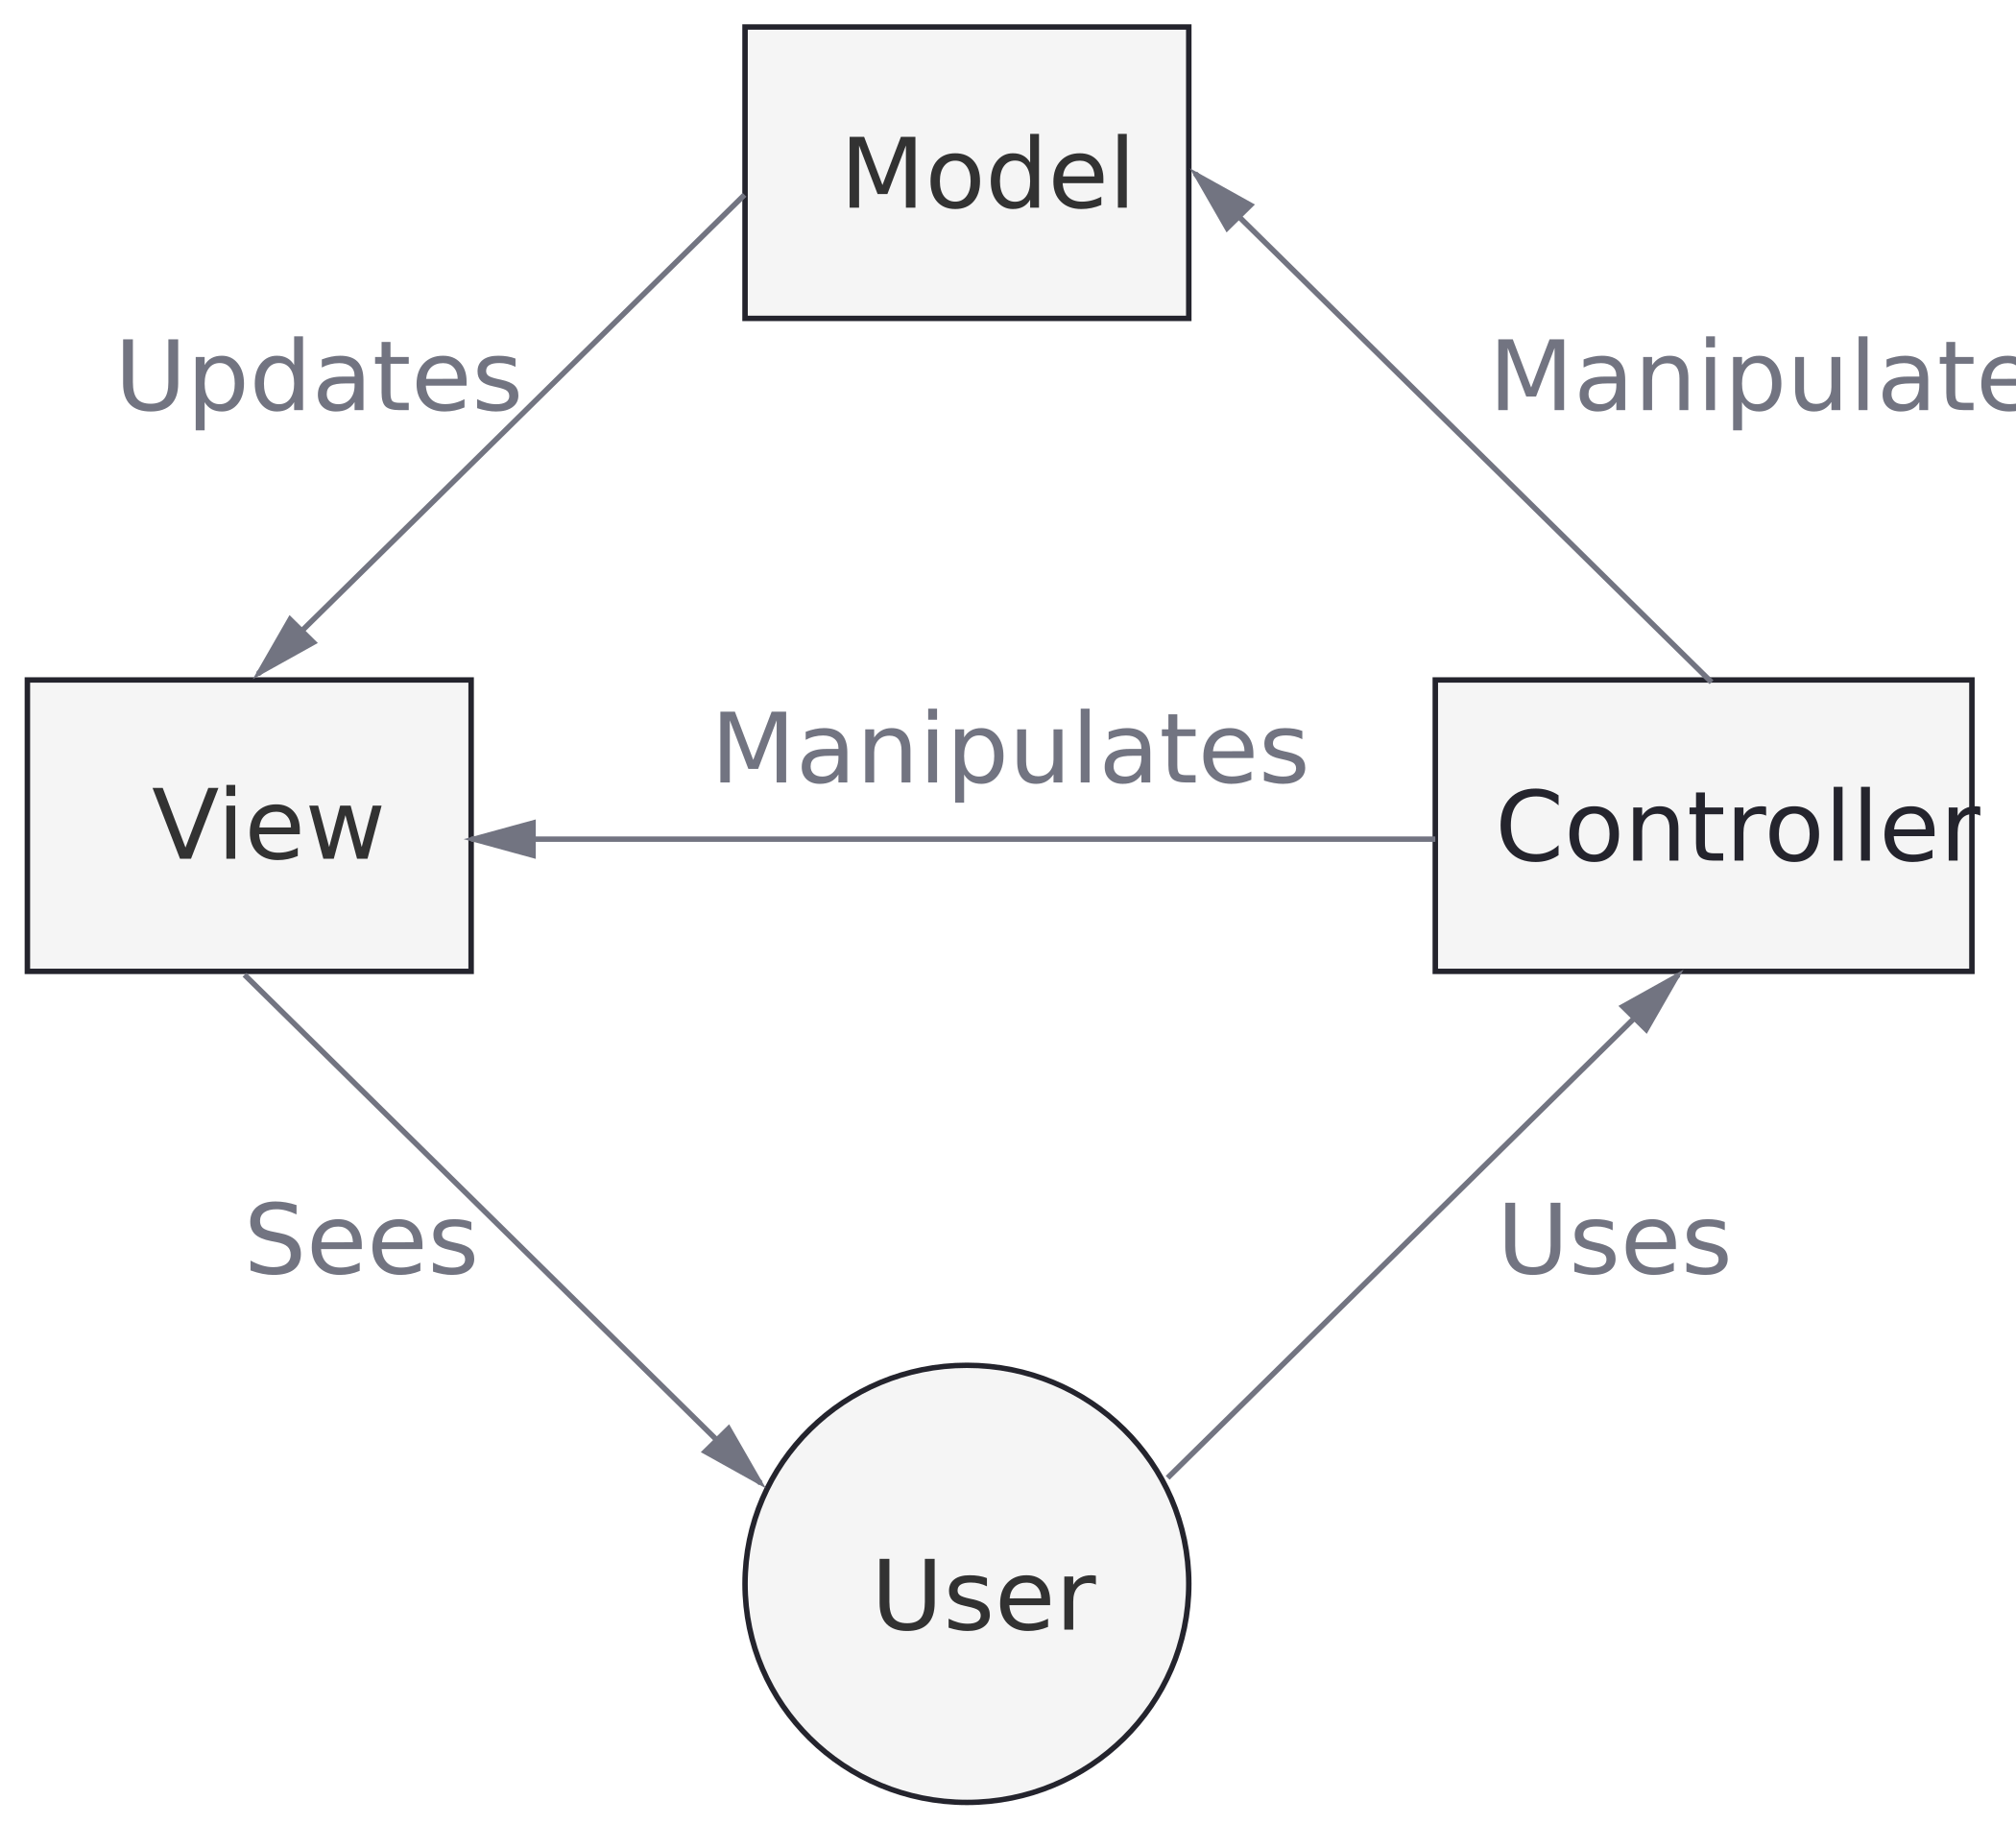
\includegraphics[height=0.5\textwidth]{./images/mvc-diagram.png}
	\caption{Model-View-Controller}
	\caption*{https://cycle.js.org/model-view-intent.html}
	\label{fig:mvc}
\end{figure}
\clearpage

\subsubsection{Mode-View-Presenter}
Das nächste im Bunde ist Model-View-Presenter (MVP) aus dem Jahre 1996.
\cite{modelViewPresenterTheTaligentMikePotel1996, modelViewPresenterMartinFowler2006}
Es kann als die erste Iteration von MVC betrachtet werden, birgt dabei allerdings ein paar wesentliche 
Unterschiede. Genau wie sei Vorreiter wird es aus drei Komponenten zusammengesetzt:

\begin{itemize}
	\item \textbf{Model}: Es beinhaltet die Business Objekte und Logik die für die Ansicht von Relevanz sind. Sie kann zuständig sein für Zugriffe auf die Datenbank, das Dateisystem und Netzwerk (oft Rest API). Es hat keine direkten Zugriff auf den »Presenter« oder due »View«.
	\item \textbf{View}: Sie ist ausschließlich für die Darstellung des UI und für die Interaktion mit dem Nutzer zuständig. Sie hat keine direkten Zugriff auf den »Presenter« oder das »Model«.
	\item \textbf{Presenter}: Er beinhaltet die Business Logik der Anwendung und steht mit der »View« und dem »Model« im Austausch. Als Bindeglied steuert er die Abläufe zwischen den Beiden.
\end{itemize}
Der gravierende Unterschied zu MVC besteht darin, dass das »Model« nichts von der »View« weiß und andersrum genauso. Der »Presenter« kontrolliert die »View«, welche jegliche Ereignisse an den »Presenter« weiterleitet. Erreicht wird diese durch die Verwendung von Interfaces bzw. Verträgen zwischen den Schichten. Damit erhält keine der Komponenten die konkrete Implementation dieser, sonder eine Abstraktion. Dies führt zu einer verbesserten Modularität, da die Komponenten zu jeder Zeit ausgetauscht werden können, solange der Vertrag »erfüllt« wird.
\begin{figure}[ht]
	\centering
	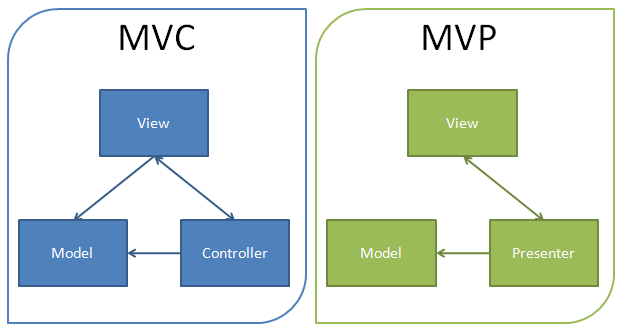
\includegraphics[height=0.45\textwidth]{./images/mvp-vs-mvc.png}
	\caption{MVC vs. MVP}
	\caption*{Source: https://i.imgur.com/xbeB5.png}
	\label{fig:mvc}
\end{figure}
\clearpage

\subsection{Historie \& Grundlegendes}
Model-View-Intent (MVI) ist eine weiteres Entwurfsmuster, welches der Feder von André (Medeiros) Staltz entstammt. Er stellte dieses auf einer Javascript Konferenz im Jahre 2015 vor
\cite{modelViewIntentIntroduction}. Es gehört damit zu den jüngsten seiner Art.
Seine ursprüngliche Anwendung fand es in dem ebenfalls von André Staltz geschaffenen Framework »CycleJs«, hat seit der Artikelreihe von Hannes Dorfmann in 2016
\cite{modelViewIntentOnAndroidHannesDorfmann2016}
aber auch den Sprung in die Welt von Android vollbracht. MVI bezieht den Großteil seines Design aus den hier bereits vorstellten Ideen und Konzepten. Das erste Ziel ist, ähnlich wie bei MVC, Informationen zwischen zwei Welten zu übersetzten: der des digitalen Bereichs des Computers und des mentalen Modells des Benutzers. Oder anders formuliert: Das Programm muss verstehen, was der Nutzer im Sinn hat.
Der zweite, zentrale Punkt von MVI besteht in der Handhabung des Zustands der Anwendung. Hierfür ist zu klären, was genau der Zustand inne hat.
\\
\\
MVI betrachtet dafür die Interaktion zwischen einem Nutzer und Programm als einen Kreis(lauf). Betätigt der Nutzer bspw.. einen Knopf, sein Output, so gestaltet sich dieser als Input für das Programm. Dieses wiederum erzeugt einen Output (z.B. eine Meldung), welcher zum Input des Nutzers wird (hier: lesen).
\begin{figure}[ht]
	\centering
	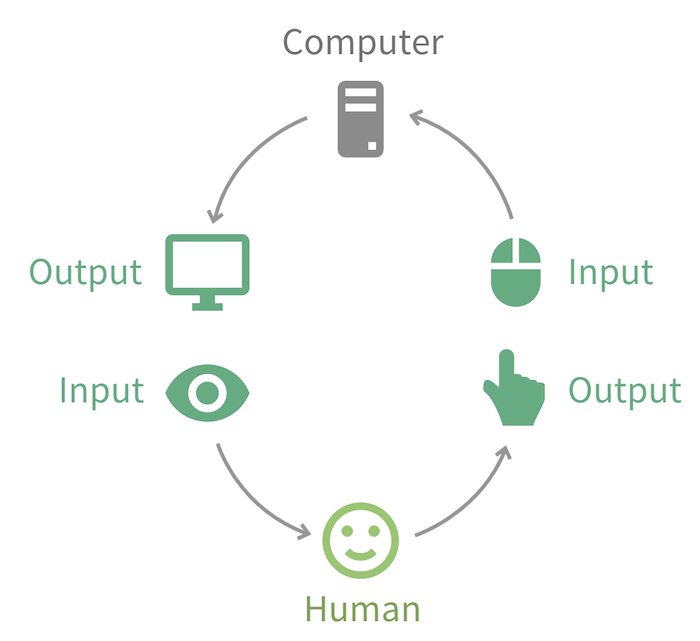
\includegraphics[height=0.5\textwidth]{./images/mvi-cycle}
	\caption{Nutzer und Computer als Input und Output}
	\caption*{Source: https://cycle.js.org/dialogue.html}
	\label{fig:userComputerInputOutput}
\end{figure}
\\
Die Grundprinzipien für den Aufbau der Architektur entspringen dabei dem beschriebenen, originalem Model-View-Controller. Das, was MVC jedoch inkompatibel für die von MVI vorhergesehenen Prozesse macht, ist die Tatsache, das der Controller proaktiv ist. Dies bedeutet, dass der »Controller« selbstbestimmt über das Model und View verfügen und diese direkt manipulieren kann. Zwangsläufig wissen die jeweiligen Komponenten auch, von welchen Komponenten sie abhängig sind. Oder anders ausgedrückt: Eine Komponente deklariert, welche anderen Komponenten sie beeinflussen, anstatt dass andere Komponenten explizit aktualisiert werden (z.B. das Modell). Dabei wird das Prinzip des unidirektionale Datenfluss verletzt, welches auch in MVI strikt verfolgt wird. 
\\
\\
Um dieses unter anderem zu erreichen, setzt MVI zusätzlich auf Reaktive Programmierung. Für MVI bedeutet reaktiv zu sein, dass jede Komponente ihre Abhängigkeiten beobachtet und auf Veränderungen dieser reagiert. Die drei Komponenten werden durch »Observables« repräsentiert, wobei der Output jeweils der Input einer anderen Komponente ist.

\subsection{Model, View \& Intent}
Fast noch wichtiger als der reaktive Ansatz ist zu verstehen, wie der Kreislauf in Figur \ref{fig:userComputerInputOutput} 
programmatisch etabliert werden kann. Betrachtet man diesen Kreis etwas genauer, so wird deutlich, dass auf einen Input immer ein Output folgt. Dieses Konzept findet man auch in der Mathematik wieder: Funktionen. Mit diesen lässt sich MVI wie folgt illustrieren:
\\
\\
\textbf{Intent}: Das I in MVI steht für »Intent« und stellt den Teil da, welches es von den anderen Entwurfsmustern unterscheidet. Das Ziel der Intent-Fuktion ist es, die Absicht des Nutzer im digitalen Kontext des Programms auszudrücken.
Ein Ereignis (oder Event), z.B. die Eingabe eines Buchstaben, kann hier der Input sein.
Der Output dieser Funktion (z.B. ein String) wird zum Input der nächsten:
\\
\\
\textbf{Model}: Die Model-Funktion nimmt das entgegen, was die Intent-Funktion produziert. Ihre Aufgabe liegt in der Verwaltung des Zustands: Sie verfügt über das Model. Sie kann daher durchaus als das zentrale Element in MVI bezeichnet werden. In Anbetracht der Tatsache, dass MVI sich als auf funktionaler Programmierung basierendes Muster versteht, ist das Model unveränderlich. Daraus ergibt sich zwangsläufig, dass für einen Zustandswechsel das Model kopiert und somit ein neues erzeugt werden muss. 
\\
Diese Funktion ist der einziges Teil des Programms, welche eine Zustandsveränderung hervorrufen kann und darf. Zusätzlich ist es der Ort, an dem auf die Business Logik der Anwendung zugegriffen wird.
\\
\\
\textbf{View}: Die View ist die letzte Funktion in der Kette, und ist zuständig für die visuelle Repräsentation des Models.
\newpage
Nimmt man alle drei Funktion zusammen, ergibt sich folgende Kette:
\begin{lstlisting}[caption={funktion}, xleftmargin=.3\textwidth, frame=false, numbers=none]
view(model(intent(input)))
\end{lstlisting}
Um den Sachverhalt zu verdeutlichten, kann dieses Beispiel in Form von pseudo-code herangezogen werden:
\begin{lstlisting}[caption={pseudo mvi implementation}, label={lst:pseudo-mvi}, language=Kotlin]
fun intent(text: String): Event {
	return EnteredTextEvent(text)
}

fun model(event: Event): Model {
	return when(event){
		is EnteredTextEvent -> {
			val newText = event.text.trim() // <-- business logic
			model.copy(text = newText) // <-- immtuable data structure
		}
	}
}

fun view(model: Model){
	textView.text = model.text 	
}

fun main(args : Array<String>) {
	view(model(intent("Hello World")))
}
\end{lstlisting}
Bei dieser Implementierung ist jedoch schnell ersichtlich, das es sich hierbei um keinen Kreis(lauf) handelt. Jede Funktion wird nur einmal aufgerufen. Es fehlt der reaktive Part, der MVI unter anderem ausmacht. Um diesen zu realisieren muss der Beispiel-Code wie folgt abgeändert werden:
\begin{lstlisting}[caption={pseudo mvi implementation},label={lst:pseudo-reactive-mvi},language=Kotlin]
// the obersvable from the textView gets passed as a parameter
fun intent(text: Observabkle<String>): Observable<Event> {
	text.map { text -> EnteredTextEvent(text) }
}

fun model(event:  Observable<Event>): Observable<Model> {
	event.map { event ->
		return when(event){
			is EnteredTextEvent -> {
			val newText = event.text.trim() // <-- business logic
			model.copy(text = newText) // <-- immtuable data structure
		}
	}	
}

fun view(model: Observable<Model>){
	// we subscribe to the model to listen for changes
	model.subscribe { model ->
		textView.text = model.text 	
	}	
}

fun main(args : Array<String>) {

	// this listens to arbitary text changes 
	val textChanges: Observable<String> = textView.changes()

	view(model(intent(textChanges))) 
}
\end{lstlisting}
Ein Punkt der in dieser Implementation noch offen bleibt, ist woher das Model kommt wie es verwaltet wird.

\subsection{Reducer}
Schaut man sich die Model-Funktion in Beispiel \ref{lst:pseudo-reactive-mvi} und ihren Inhalt genau an, so wird ein bestimmtes Muster bzw. ein sich wiederholender Ablauf erkennbar:
\\
\begin{enumerate}
	\item Die Funktion erhält ein Event 
	\item Die Funktion evaluiert das Event
	\item Die Funktion führt basierend auf dem Event (Business) Logik aus
	\item Die Funktion erzeugt ein neues Model
	\item Die Funktion gibt das neue Model zurück
\end{enumerate}
Der einzige Schritt der Fehlt, ist die Bereitstellung des derzeitigen oder des vorherigen Models. Hier kommt eine Komponente ins Spiel, die bereits in Kapitel
\ref{subsec:redux} 
angesprochen wurde: der »Reducer«. Er ist für genau den oben aufgeführten Prozess zuständig und der Platz, an dem das Model verändert wird.

\subsection{Endlicher Automat}
Wenn der in der Model-Funktion ausgeführte Code eine neues Model hervorbringt, so bleibt der Zustand entweder der Gleiche oder er verändert sich. Unabhängig davon geht der Zustand in den selbigen oder in einen neuen Zustand über: es kommt zu einem sogenannten Zustandsübergang. Aber nicht nur das lässt sich aus dem gezeigten Beispiel ableiten; es sind noch weitere Schlussfolgerungen zulässig:
\\
\begin{itemize}
	\item Es gibt immer einen Anfangszustand bzw. Startzustand
	\item Es gibt eine endliche Anzahl von Zuständen
	\item Es gibt eine beliebe Menge von Endzuständen
	\item Es gibt immer nur einen Zustand, in dem sich die Anwendung befinden kann
\end{itemize}
\bigskip
Die oben genannten Punkte lassen sich anhand eines weiteren Beispiels besser erläutern: Man nehme an, dass sich auf einem Bildschirm ein Textfeld und ein dazugehöriger Knopf befindet. Das Textfeld ist anfänglich leer und der Knopf deaktiviert. Dieser kann nur aktiviert werden, wenn eine Eingabe im Textfeld erfolgt. Hiermit ist der Startzustand des Knopfs »deaktiviert« (z0). Gibt der Nutzer im Textfeld einen Text ein, so wird der Knopf aktiviert. Dieses Ereignis ist der bereits angeführte Zustandsübergang.
Gleichzeitig wird ein Endzustand erreicht (z1) - weitere Eingaben führen zu keinem neuem Zustand.
Die Beschreibungen z1 und z2 dienen hierbei als das Eingabealphabet und zeigen die Menge von potenziellen Ereignissen auf.
\begin{figure}[ht]
	\centering
	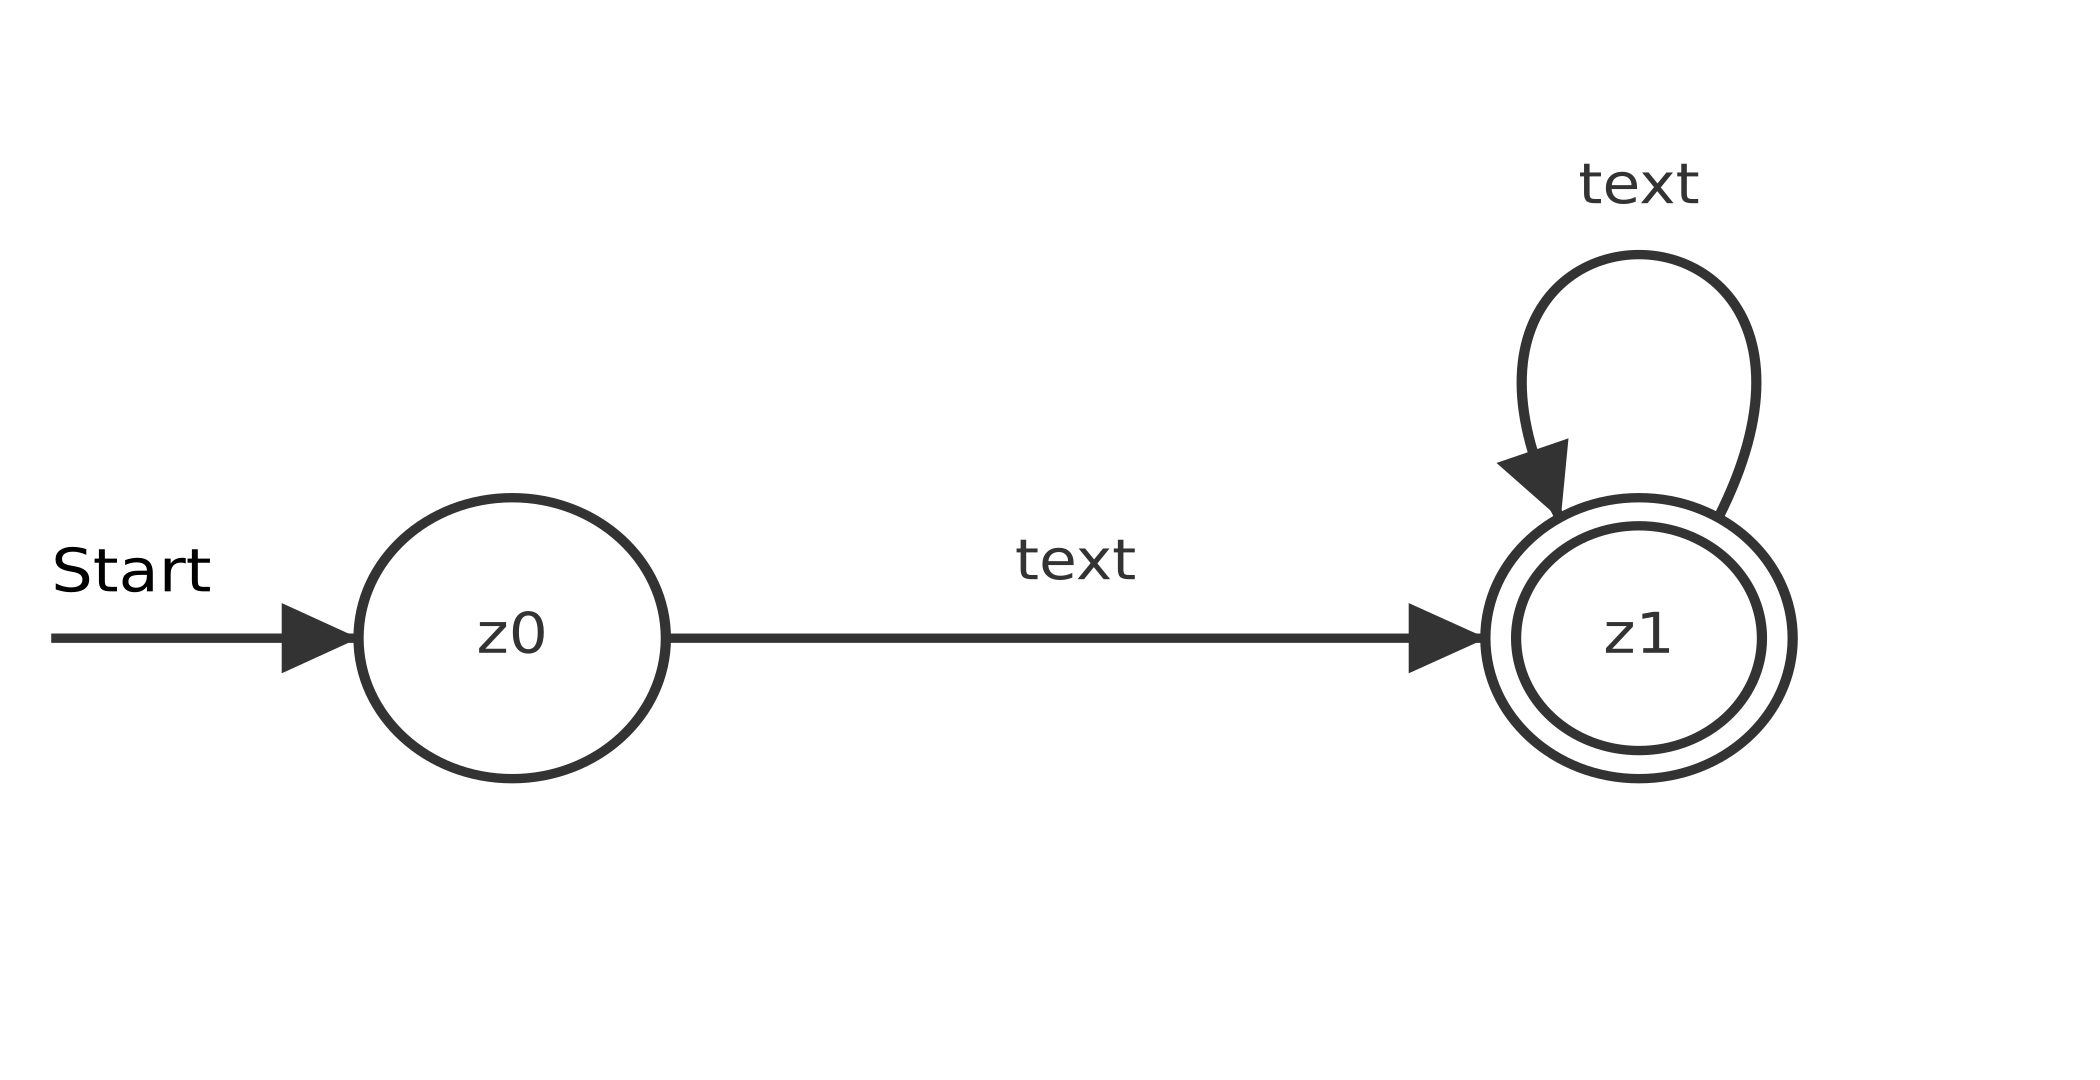
\includegraphics[height=0.35\textwidth]{./images/out}
	\caption{Endlicher Automat}
	\label{fig:endlicherAutomat}
\end{figure}
\\
Dieses Konzept ist in der Informatik bekannt als "Endliche Automaten". Ihr Ziel ist es, ein bestimmtes Verhalten (wie das obige) zu Modellieren und unter anderem visuell in Form von Abbildung
\ref{fig:endlicherAutomat} 
zu präsentieren.